\chapter{Hardware Environment}
\thispagestyle{empty}
\label{sec:hw-env}
\newcommand{\LocHWfig}{\Origin/user-code/hw-env/figures}
\newcommand{\LocHWscicode}{\Origin/user-code/hw-env/scilab}
\newcommand{\LocHWscibrief}{Origin/user-code/hw-env/scilab}
\newcommand{\LocHWardcode}{\Origin/user-code/hw-env/arduino}
\newcommand{\LocHWardbrief}{\tt Origin/user-code/hw-env/arduino}
\newcommand{\LocSH}{\Origin/tools/shield}
%\newcommand{\LocSHbrief}{{\tt Origin/tools/shield}}
\newcommand{\LocSHbrief}[1]{{\tt Origin/tools/shield/#1}, see \fnrefp{fn:file-loc}}

In this book, we shall use an \arduino\ board and associated circuitry
to perform several experiments on data acquisition and control. This
chapter will briefly take you through the hardware environment needed
to perform these experiments. We will start with the introduction to a
microcontroller followed by a brief on Open Source Hardware. Then, we
shall go through the history and hardware specifications of the
Arduino Uno board and the schema and uses of the Shield provided in
the kit.


\section{Microcontroller}
A microcontroller is a ``smart'' and complex programmable digital circuit
that contains a processor, memory and input/output peripherals on a
single integrated circuit. Effectively, it can function as a small
computer that can perform a variety of applications. A few of these
day to day applications include:
\begin{itemize}
\item Automotive: Braking, driver assist, fault diagnosis, power
  steering
\item Household appliances: CD/DVD players, washing machines,
  microwave ovens, energy meters
\item Telecommunication: Mobile phones, switches, routers, ethernet
  controllers
\item Medical: Implantable devices, MRI, ultrasound, dental imaging
\item General: Automation, safety systems, electronic measurement
  instruments
\end{itemize}

\subsection{Organization of a Microcontroller}
In this section, we will give a brief overview of the organization of
a typical microcontroller.  A microcontroller consists of three major
components, namely, Processor, Memory and Peripherals. The basic block
diagram of a microcontroller is shown in \figref{micro-arch}. We shall
briefly review the functionality of each block.

\begin{figure}
\centering
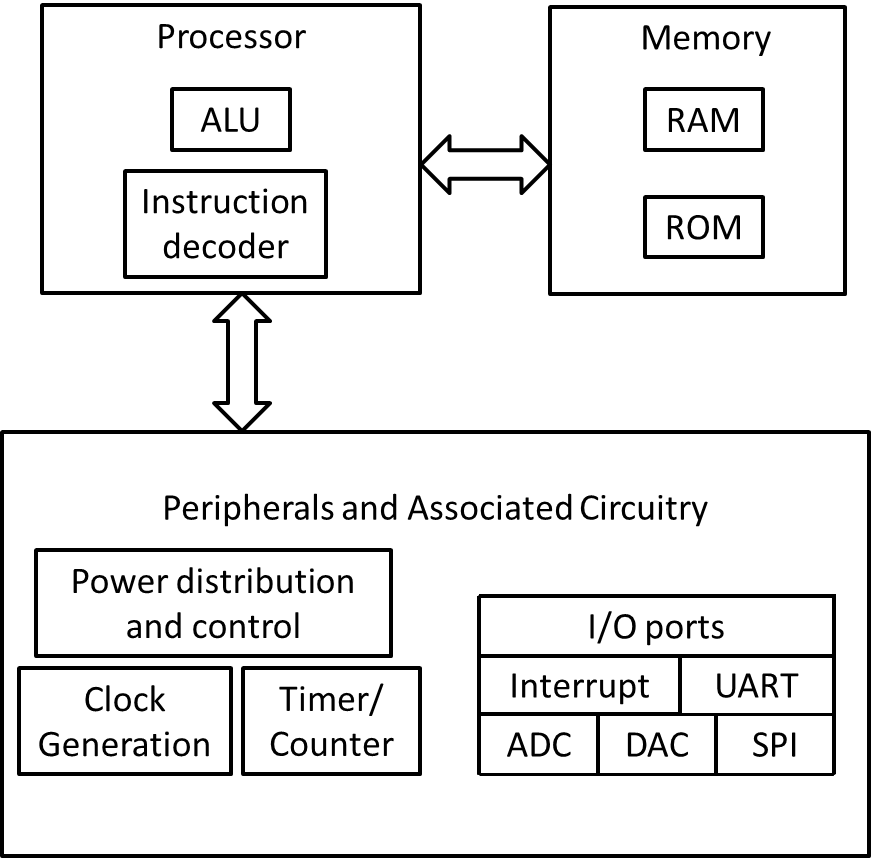
\includegraphics[width=\lgfig]{\LocHWfig/miccontblk.png}
\caption{Functional block diagram of a microcontroller}
\label{micro-arch}
\end{figure}

\begin{description}
\item {Processor:} It is also known as a Central Processing Unit
  (CPU).  A processor is the heart of any computer/embedded
  system. The applications running on these systems involve arithmetic
  and logic operations. These operations are further simplified into
  instructions and fed to the processor.  The Instruction decoder
  decodes these instructions while arithmetic and logic operations are
  taken care of by an Arithmetic and Logic Unit (ALU). A modern day
  CPU can execute millions of instructions per second (MIPS). 

\item {Memory:}
A computer memory, usually a semiconductor device, is used to hold data and instructions. Depending on the make, it could be volatile or non-volatile in nature. There are different types of memory:
\begin{enumerate}
\item Read Only Memory (ROM): It is a non-volatile storage entity. It
  is used in computers, phones, modems, watches and other electronic
  devices. A program is typically uploaded (flashed) to ROM through PC.
  Its content cannot be modified; it can only be erased and flashed
  using compatible tools.
\item Random-access Memory: RAM is a volatile storage entity. It is
  used by CPU to store intermediate data during the execution of a
  program. RAM is usually faster than ROM.   
\item Electronically Erasable Programmable Read-Only Memory: EEPROM is
  an optional non-volatile storage entity. It can be erased and
  written by the running program.  For example, it can be used to
  store the values of a temperature sensor connected to the microcontroller.
\end{enumerate}
\end{description}

\subsection{Microcontroller Peripherals}
Microcontrollers have a few built-in peripherals.  In this section, we
will review them briefly.

\begin{description}
\item {Clock:} A complex digital circuit, such as the one that is
  present in a microcontroller, requires a clock pulse to
  synchronize different parts of it.  The clock
  is generated through internal or external crystal oscillator. A
  typical microcontroller can execute one instruction per clock
  cycle (time between two consecutive clock pulses).

\item {Timer/Counter:} A timer is a pulse counter. A timer circuit is
  controlled by registers. An 8-bit timer can count from 0 to 255. A
  timer is primarily used to generate delay, and could be configured
  to count events.
    
\item{Input/Output Ports:} I/O ports correspond to physical pins on
  the microcontroller. They are used to interface external peripherals. A
  port can be configured as input or output by setting bits in I/O
  registers. Each pin can be individually addressed too.

\item{Interrupts:} An interrupt to the CPU suspends the running program
  and executes a code block corresponding to it. After serving/attending
  interrupts, the CPU resumes the previous program and continues. An
  interrupt could be originated by the software or the hardware. A
  hardware interrupt normally has a higher priority.

\item {Universal Asynchronous Receiver/Transmitter (UART):} UART is a
  standard microcontroller peripheral to communicate with external
  serial enabled devices. It has two dedicated pins to be used as
  Rx (Receiver) and Tx (Transmitter).  The baud rate defines the speed
  of the UART and can be configured using registers.

\item {Analog to Digital Converter (ADC):} Most of the signals around
  us are continuous. Digital circuits cannot process them. An ADC
  converts them into digital signals. The resolution of the ADC
  determines the efficiency of conversion. For example, a 10-bit
  resolution of the ADC relates to 1024 values per sample. This is
  shown pictorially in \figref{resolution}. Higher resolution relates
  to better translation of an analog signal.

\begin{figure}
  \centering
  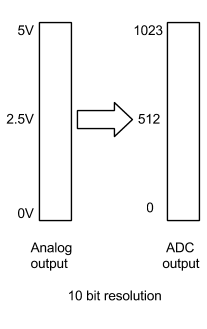
\includegraphics[width=\tnfig]{\LocHWfig/resolution.png}
  \caption{ADC resolution}
  \label{resolution}
\end{figure}

\item {Digital to Analog Converter (DAC):} Digital output of the CPU is
  converted to analog signals using the pulse width modulation (PWM)
  technique. The output of a DAC is used to drive analog devices and actuators.

\item {Serial Peripheral Interface (SPI):} SPI is a synchronous 4 wire
  serial communication device. It requires a master and slave
  configuration. The SPI peripheral has dedicated pins and marked
  as:
  \begin{enumerate}
  \item SCLK (from Master)
  \item MOSI (Master out, Slave input)
  \item MISO (Master Input, Slave output)
  \item Slave select (Active when 0V, originates from Master)
  \end{enumerate}

\item {Firmware:} Firmware is an application that configures the
  hardware. It is programmed to a non-volatile memory such as ROM,
  EPROM (Erasable Programmable ROM). This concept is used in computer
  BIOS and embedded devices.  In a microcontroller setup, a firmware
  file contains addresses and hexadecimal values.

\item{Interfacing:} Some of the popular connections with microcontrollers include,
  \begin{enumerate}
  \item Digital input devices: Switch, keypad, encoder, multiplexer,
    touchscreen
  \item Digital output devices: LED, LCD, relay, buzzer
  \item Digital input and output devices: RTC (Real Time Clock),
    SD Card, external ROM
  \item Analog input devices: Audio, sensor, potentiometer
  \item Analog output devices: Brightness control, speaker
  \item Serial communication (UART): GSM, GPS, Zigbee, Bluetooth
  \end{enumerate}
\end{description}

\section{Open Source Hardware (OSHW)}
\label{sec:oshw}
In this section, we will introduce the reader to Open Source Hardware
(OSHW), which is 
\emph{defined} as follows \cite{oshw-ref}:
\begin{quote}
Open source hardware is a hardware whose design is made publicly
available so that anyone can study, modify, distribute, make, and sell
the design or hardware based on that design...
\end{quote}
The OSHW website \cite{oshw-ref} gives additional conditions to be
fulfilled before the hardware can be called OSHW.  It also argues why
we should promote and contribute to OSHW.  The logo of OSHW is given
in \figref{fig:OSHW-logo} \cite{OSHW-logo-ref}.
\begin{figure}
\centering

\includegraphics[width=1in]{\LocHWfig/OSHW-138px.png}
\caption{The logo of Open Source Hardware}
\label{fig:OSHW-logo}
\end{figure}
The open-source hardware initiative is popular in the electronic,
computing hardware and automation industry.  Here are some examples of
open-source hardware projects:
\begin{enumerate}
\item The ``open compute project'' at Facebook shares the design of
  data center products.
\item Beagle board, Panda board, OLinuXino are ARM based development
  boards.
\item ``Open Graphics Project (OGP)'' releases the designs of
  graphics card.
\item ``ArduCopter'' is a UAV (unmanned aerial vehicle) created by
  the \emph{DIY Drones} community.
\item ``NetFPGA'' is a prototyping of computer network devices.
\item ``OpenROV'' project (Open Source Remotely Operated Vehicle)
  aims at affordable underwater exploration.
\item ``OpenMoko'' project set the foundation for open-source mobile
  phones. ``Neo 1973'' was the first smartphone released in 2007
  with Linux based operating system, it had 128MB RAM and 64MB ROM.
\end{enumerate}

Companies like Adafruit Industries, Texas Instruments, Solarbotics,
Sparkfun electronics, MakerBot industries and DIY Drones have proven
the power of OSHW with their revenues.  Nevertheless, collaborative
innovation using OSHW is yet to establish itself in the mainstream.  But
the trend has certainly started and is going strong.  There are now
many robotics startups taking full use of OSHW.

\section {Arduino}
Arduino is an open-source microcontroller board and a software
development environment. Arduino language is a \emph{C} like
programming language which is easy to learn and understand.  Arduino
has two components, open source hardware and open source software.  We
will cover the basics of the Arduino hardware in this section.

\subsection{Brief History}
Arduino project was started at the \emph{Interaction Design Institute
  Ivrea} in Ivrea, Italy. The aim was to create a low-cost
microcontroller board that anyone with little or no background domain
knowledge can design and develop. Arduino uses expansion circuit
boards known as \emph{shields}. Shields can provide GPS, GSM,
Bluetooth, Zigbee, motor and other functionality.

Within the first two years of its inception, the Arduino Team sold
more than 50,000 boards. In 2011, Google announced \emph{The Android
Open Accessory Development Kit (ADK)}, which enables the Arduino boards to
interface with Android mobile platform.

Today Arduino is the first choice for electronic designers and
hobbyists. There are  more than 13 official variants of Arduino and
many more third-party Arduino software compatible boards.  

\subsection{Arduino Uno Board}
There are different Arduino boards for different requirements. All
original Arduino boards are based on ATMEL microcontrollers.  In this
section, we will briefly discuss the \arduino\ board, the most popular
Arduino board.  We will illustrate all applications using the
\arduino\ board in this book.

Based on ATmega328, the \arduino\ board has 14 digital input/output
pins, 6 analog inputs, 6 PWM pins, a 16 MHz ceramic resonator, a power
jack, an ICSP (In-Circuit Serial Programming) header, and a reset
button. It has an on-board USB to serial converter and can be connected
to a PC using a USB cable.  \figref{arduino} has a picture of this board
\cite{uno-ref}.  \tabref{micro-table} has the specifications of the
\arduino\ board.

\begin{figure}
  \centering
  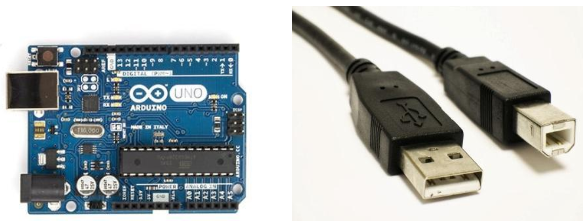
\includegraphics[width=\hgfig]{\LocHWfig/arduino.png}
  \caption{Arduino Uno Board}
  \label{arduino}
\end{figure}

\begin{table}
\begin{center}
\begin{tabular}{ || l | c || r }
 \hline		
{\bf Parameter} & {\bf Value} \\ \hline	
 Microcontroller & ATmega328P\\
Operating Voltage & 5V\\
Input Voltage (recommended) & 7-12V\\
Input Voltage (limits) & 6-20V\\
Digital I/O Pins & 14 (of which 6 provide PWM output)\\
Analog Input Pins & 6\\
DC Current per I/O Pin & 20 mA\\
DC Current for 3.3V Pin & 50 mA\\
Flash Memory & 32 KB (ATmega328), 0.5 KB used by bootloader\\
SRAM & 2 KB (ATmega328)\\
EEPROM & 1 KB (ATmega328)\\
Clock Speed & 16 MHz\\
Length & 68.6 mm\\
Width & 53.4 mm\\
Weight & 25 g\\
 \hline 
\end{tabular}
\caption{Arduino Uno hardware specifications}
\label{micro-table}
\end{center}
\end{table}

Another popular board is Arduino Mega board.  Based on
ATmega2560, this board has almost double the size of program
memory (ROM) compared to Arduino Uno.  It also has extra serial ports,
digital and PWM pins.  \figref{mega} has a picture of this board
\cite{mega-ref}. 
\begin{figure}
  \centering
  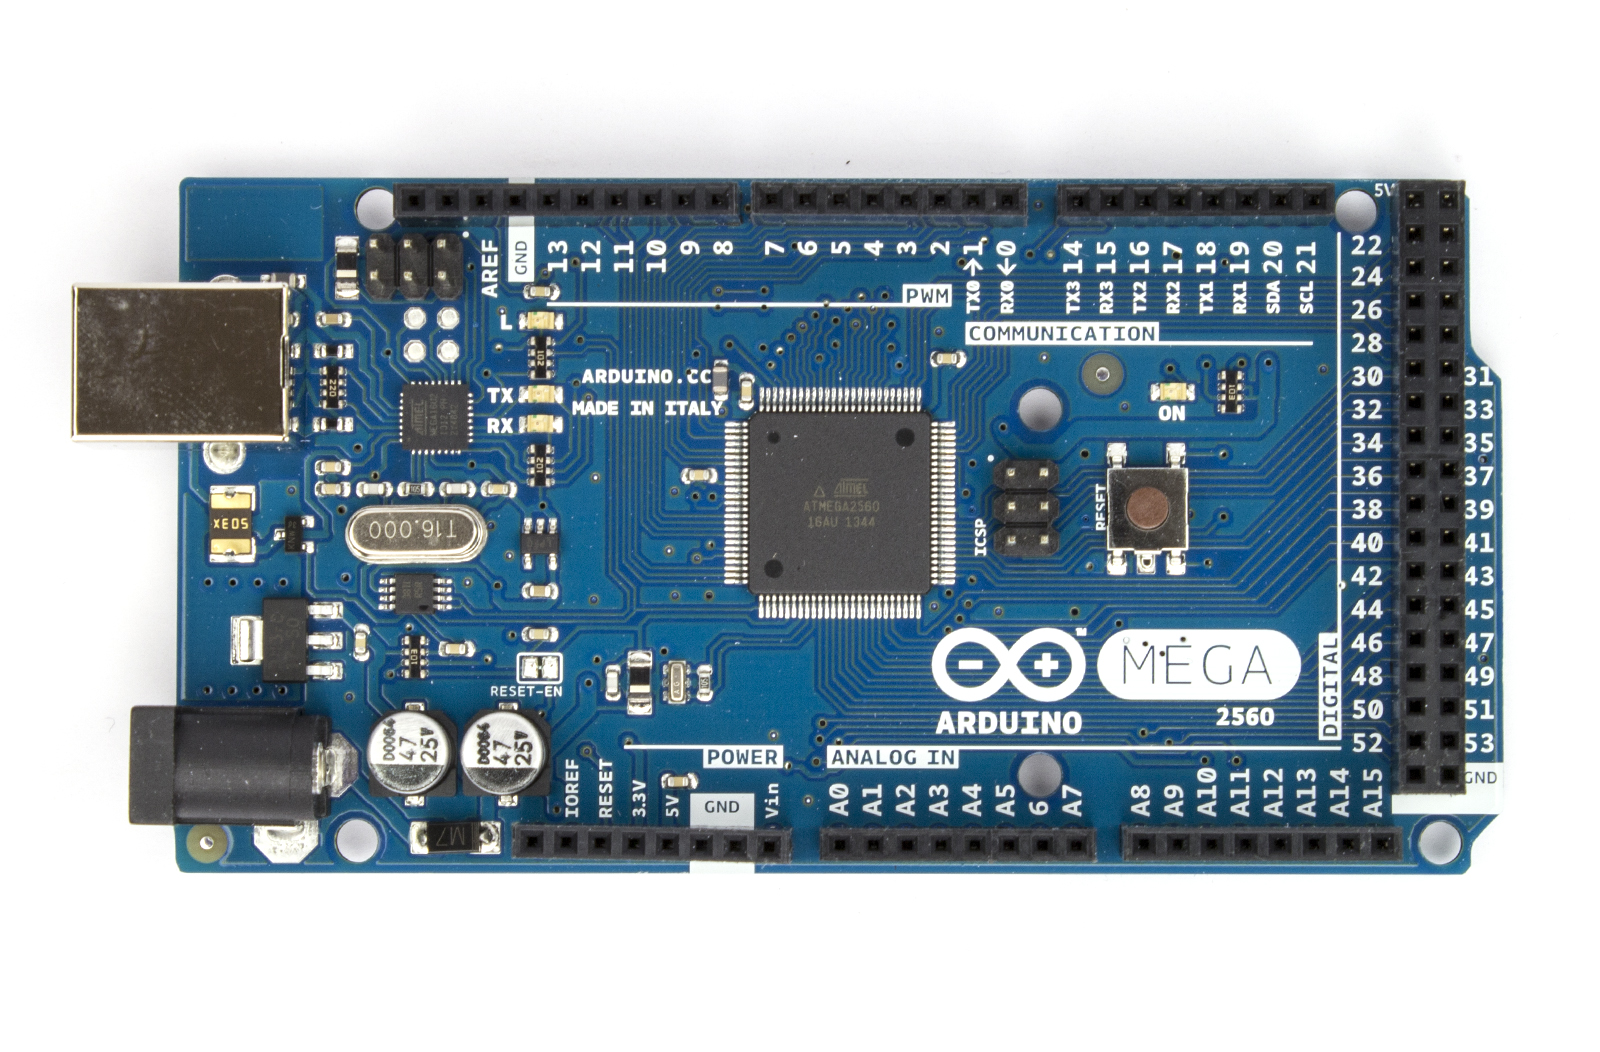
\includegraphics[width=\lgfig]{\LocHWfig/mega.jpg}
  \caption{Arduino Mega Board}
  \label{mega}
\end{figure}

Yet another popular board is LilyPad Arduino, a small circular
board for fabric designers. It can be stitched with conductive thread,
and it supports sensors and actuators.  \figref{lily} has a picture of
this board \cite{lily-ref}.
\begin{figure}
  \centering
  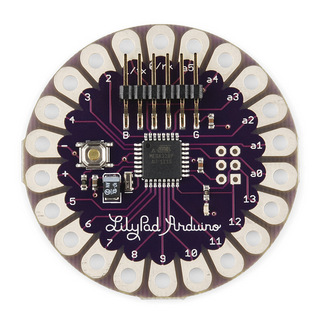
\includegraphics[width=\smfig]{\LocHWfig/lily.jpg}
  \caption{LilyPad Arduino Board}
  \label{lily}
\end{figure}

There are other similar configuration boards with different form
factors, such as Arduino Fio, Arduino Mini, Arduino Nano, Arduino
Duemilanove, Arduino serial and so on.

\subsection{Popular Arduino Projects}
Arduino is intuitive and it's easy to setup and use. That's why people around the globe 
are using Arduino in innovative ways. We list a few of these projects to give a 
flavor of some of these interesting applications.

\paragraph{Arduino phone:} An Arduino connected with a graphic LCD and a
GSM shield. This low-tech phone, shown in \figref{arduino-phone} can
be built in a few hours \cite{phone-ref}.  
\begin{figure}
  \centering
  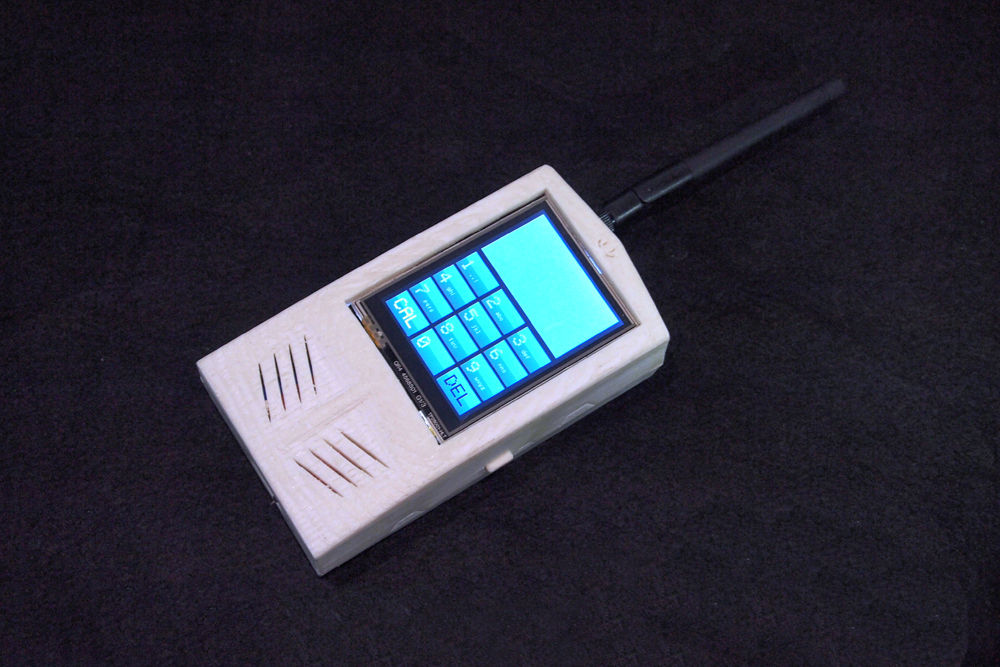
\includegraphics[width=\smfig]{\LocHWfig/arduino-phone.jpg}
  \caption{Arduino Phone}
  \label{arduino-phone}
\end{figure}

\paragraph{Candy sorting machine:} As the name suggests, this machine 
can sort candy based on its color to separate jars \cite{candy-ref}.

\paragraph{3D printers:} There are open-source 3D printers based on
Arduino and  Raspberry Pi. Although 3D printers, shown in \figref{3dprinter},
 are relatively slow and lack precision, they can be ideal for building prototypes by
hobbyists \cite{3d-printer-ref}.
\begin{figure}
  \centering
  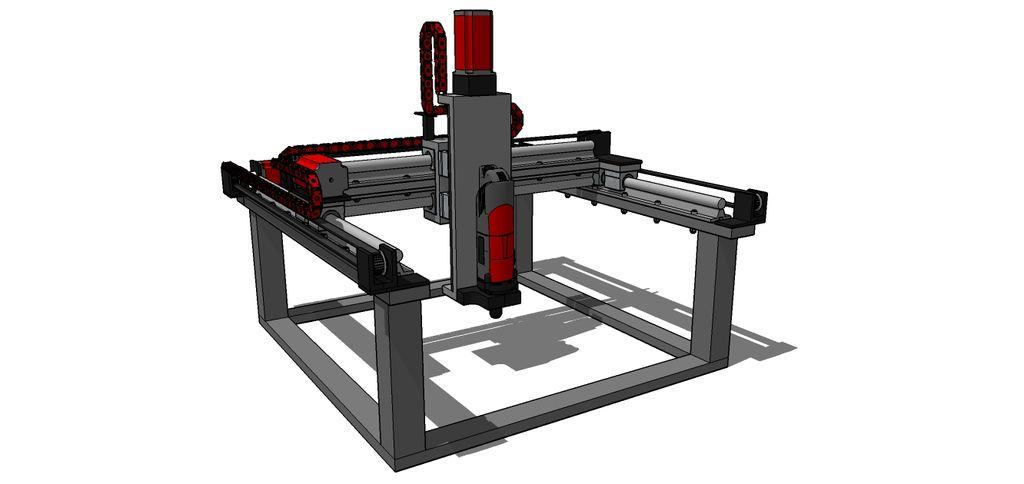
\includegraphics[width=\smfig]{\LocHWfig/arduino-3d-printer.jpg}
  \caption{3D printer}
  \label{3dprinter}
\end{figure}

\section{Shield}
The shield that we use in this book is a modified version of the Diyode Codeshield 
board \cite{shield-ref}, which makes it easy to perform
experiments on the Arduino Uno board.  The shield is a printed circuit
board (PCB) with a large number of sensors, already wired and hence,
ready to use.  It obviates the need for a breadboard as an
intermediate tool for electronics circuit prototyping, which is quite
cumbersome for beginners.  The shield provides the user a faster way
of circuit prototyping without worrying much about troubleshooting.

The numbering on the shield is identical to that on
the \arduino\ board.  The shield fits snugly on to the \arduino\
board, obviating the need to do the wiring in many experiments.  One
can even say that shields have made the hardware experiments involving
Arduino boards as easy as writing software.

All the experiments in this book have been verified with the use of a
modified version of Diyode Codeshield, as mentioned above.  We make
available all the required information to make a shield, thus making
this an OSHW, see \secref{sec:oshw}.

We now explain where the required files to make our shield are given.
The gerber file to make the shield is given in
\LocSHbrief{gerber-V1.2}.  The image of the PCB file is given in
\figref{fig:PCB-image}, which also helps locate the PCB file.
\begin{figure}
\centering
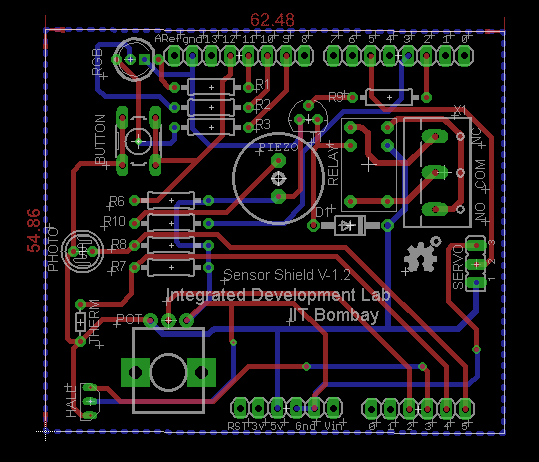
\includegraphics[width=\smfig]{\LocSH/pcb_board_V1p2.png}
\caption[PCB image of the shield]{PCB image of the shield.  The PCB
  file can be found at \LocSHbrief{shield-V1p2.brd}.}
\label{fig:PCB-image}
\end{figure}
The pictorial representation of the schematic for the shield is given
in \figref{fig:sch-shield}, which also helps locate the schematic of
the shield.
\begin{figure}
\centering
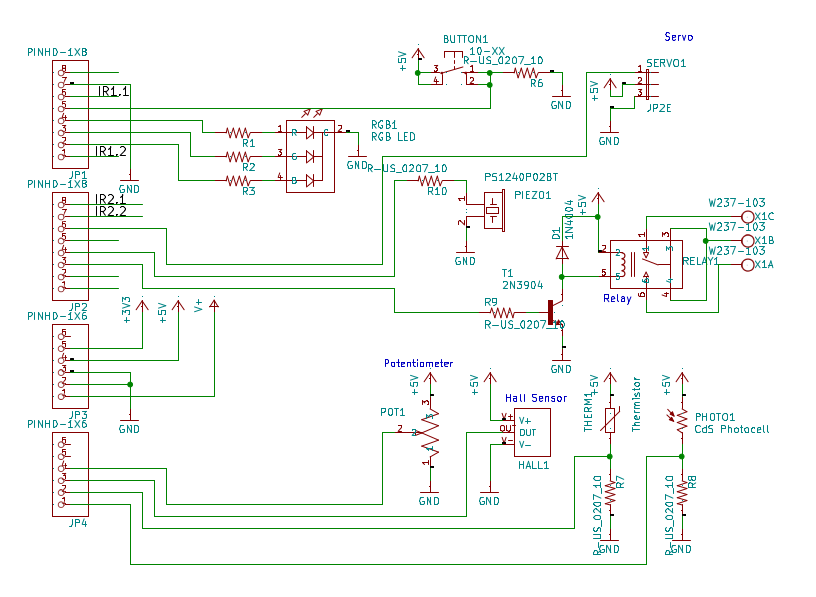
\includegraphics[width=\linewidth]{\LocSH/shield-V1p2.png}
\caption[Pictorial representation of the schematic of the
shield]{Pictorial representation of the schematic of the shield.  The 
actual schematic can be found at 
\LocSHbrief{shield-V1p2.sch.}}
\label{fig:sch-shield}
\end{figure}
A photograph of the PCB after fabrication is given in
\figref{fig:shield-photo}. 
\begin{figure}
\centering
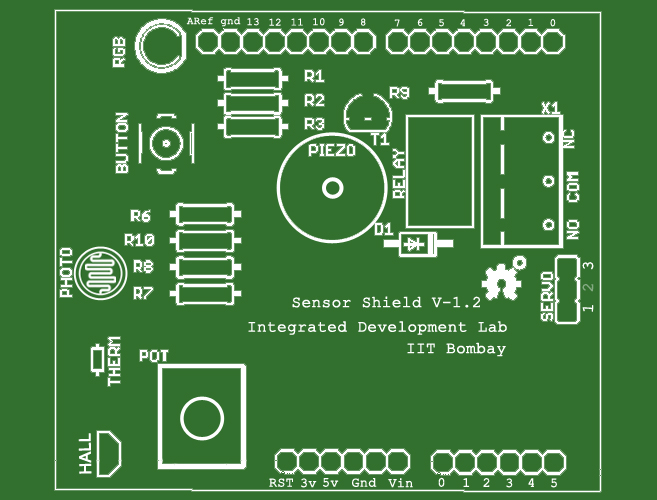
\includegraphics[width=0.6\linewidth]{\LocSH/shield-V1p2.jpg}
\caption[PCB of the
shield]{PCB of the shield.  The 
actual image can be found at 
\LocSHbrief{shield-V1p2.sch.}}
\label{fig:shield-photo}
\end{figure}

The values of the various components used in the shield are given in 
\tabref{tab:shield-values}.  
\begin{table}
\centering
\caption{Values of components used in the shield}
\label{tab:shield-values}
\begin{tabular}{|l|l|c|} \hline
Name & Description & Quantity \\ \hline
R1 & $100\Omega$ Resistor (Br-Bl-Br) & 1 \\ 
R2, R3, R4 & $91\Omega$ Resistor (Wt-Br-Bl) & 3 \\
R5, R6, R7, R8 & $10K\Omega$ Resistor (Br-Bl-Or) & 4 \\
R9 & $1K\Omega$ Resistor (Br-Bl-Rd) & 1 \\
D1 & Diode & 1 \\
Relay & Relay & 1 \\
X1 & Terminal block & 1 \\
Piezo & Piezo & 1 \\ 
LED 1 & LED - 2 lead & 1 \\
LED 2 & RGB LED & 1 \\
T1 & Transistor & 1 \\
SWITCH & Switch & 1 \\
BUTTON, RESET & Push button & 2 \\
PHOTO & Photo resistor & 1 \\
HALL & Hall effect sensor & 1 \\
POT & Potentiometer & 1 \\
% ENC & Rotary encoder & 1 \\
THERM & Thermistor & 1 \\
SERVO & Servo & 1 \\
SERVO-PARTS & Servo parts & 1 \\
% NUT, BOLT & Nut, bolt & 2 \\
HEADER & 6x pin header & 2 \\
HEADER & 8x pin header & 2 \\
\hline
\end{tabular}
\end{table}
\tabref{shield-table} provides information about various sensors,
components on Shield and its corresponding Pin on Arduino Board
\cite{shield-ref}.  
\begin{table}
\centering
\caption{Information on sensors and pin numbers}
\label{shield-table}
\begin{tabular}{ || l | c || r }
 \hline		
{\bf Shield components} & {\bf Arduino pin}\\ \hline	
RGB LED BLUE & Digital Pin 9\\
RGB LED GREEN & Digital Pin 10\\
RGB LED RED & Digital Pin 11\\
PUSH BUTTON & Digital Pin 12\\
THERMISTOR & Analog Pin 4\\
RELAY  & Digital Pin 2\\
POTENTIOMETER & Analog Pin 2\\
PHOTORESISTOR (LDR) & Analog Pin 5\\
HALL EFFECT SENSOR & Analog Pin 3\\
BUZZER & Digital Pin 3\\
 \hline 
\end{tabular}
\end{table}
A picture of the completed shield is in \figref{shield}.
\begin{figure}
  \centering
  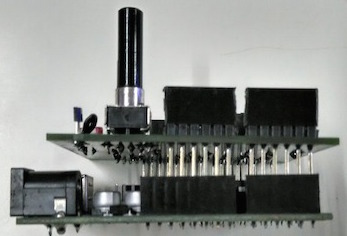
\includegraphics[width=\linewidth]{\LocHWfig/shield-crop.jpg}
  \caption{Picture of the shield with all components}
  \label{shield}
\end{figure}

\section{Experimental Test Bed}
We experimented with the contents of this book with the
following list.  We will refer to this as a \emph{kit} in the rest of
this book.
\begin{enumerate}
\item \arduino\ board
\item Shield containing
\begin{enumerate}
\item LED
\item LDR
\item Push Button
\item Thermistor
\end{enumerate}
\item DC motor and its controller board
\item Servo motor
\item Energy meter with Modbus interface
\end{enumerate}

The \arduino\ board is easily available in the market.  The shield is
designed by us.  Details of most of these units are provided in the
previous sections.  Information on all of these is available in the
file, mentioned in \fnref{fn:file-loc}.


